\documentclass[10pt]{article}

\usepackage{fullpage}
\usepackage[margin=2cm]{geometry}
\usepackage[pdftex]{graphicx}
\usepackage{float}

\begin{document}

\title{\vspace{-2cm}Programming in C: Group 21 Project Report}
\author{\small Alexander CLARKE, Qiang FENG, Jordan SPOONER, Laurence SQUIRES}

\maketitle

\section{ARM11 Emulator and Assembler}

The folder structure for the project is as follows:

\begin{itemize}
\item \texttt{emulate\_utils/} contains the files containing the constants, structs and helper functions for our emulator.
\item \texttt{assemble\_utils/} contains the files containing the constants, structs and helper functions for our assembler.
\end{itemize}

\begin{figure}[H]
\begin{minipage}{0.6\linewidth}

\subsection{Emulator Implementation}

We structured our emulator as follows:

\begin{itemize}
\item \texttt{emulate.c} contains the function \texttt{main}, which takes a single parameter of the filename containing ARM11 object code. \texttt{main} calls the function \texttt{load\_file} from \texttt{toolbox.h} to load the file into memory, \texttt{decode\_instruction} and \texttt{execute} from \texttt{emulate\_utils/decode.h} and \texttt{emulate\_utils/execute.h} respectively, for the main fetch-decode-execute cycle, and \texttt{print\_system\_state\_compliant} from \texttt{emulate\_utils/print\_compliant.h}, which prints the registers and non-zeroed memory in a format which passes the automated tests.
\item \texttt{unit\_tests.c} contains a suite of simple tests that check the functionality of each of the called functions. Rather than using a unit testing framework, we opted for a simple macro and use of \texttt{assert.h} to check our functions work as documented.
\item \texttt{emulate\_utils/print\_compliant.c} contains functions for printing output to \texttt{stdout} in a way that passes test cases. It defines \texttt{print\_system\_state\_compliant} as well as several helper functions.
\end{itemize}

\end{minipage}
\hspace{0.05\linewidth}
\begin{minipage}{0.35\linewidth}

\centering
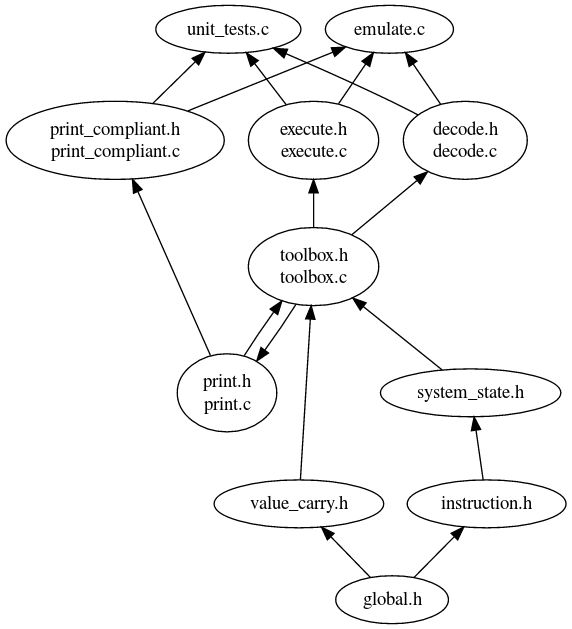
\includegraphics[scale=0.3]{Checkpoint/emulate.png}
\caption{Dependency Graph for \texttt{emulate.c}}

\end{minipage}
\end{figure}

\begin{itemize}
\item \texttt{emulate\_utils/print.c} contains functions for printing output that is extremely helpful for debugging. Some of these functions are also called by the compliant printing functions. Setting \texttt{COMPLIANT\_MODE} to \texttt{false} in \texttt{global.h} uses these functions instead of the compliant ones. The output no longer passes tests, but more details, such as the most recently fetched and decoded instructions, will be printed.
\item \texttt{emulate\_utils/decode.c} contains the function \texttt{decode\_instruction} and helper functions to decode each type (data processing, multiply, single data transfer, branch) of instruction.
\item \texttt{emulate\_utils/execute.c} contains the function \texttt{execute} and helper functions for each type of instruction.
\item \texttt{toolbox.c} contains a number of useful helper functions used throughout the code. It includes the function \texttt{load\_file}, as well as \texttt{exit\_program}, which prints the current system state before exiting cleanly, functions to read and write to memory (\texttt{get\_word\_compliant} and \texttt{set\_word} respectively), functions for working with two's complement numbers, and the \texttt{shifter} function, which emulates a shifter. \texttt{get\_word\_compliant} and \texttt{set\_word} already implement the requirements of Part III, by printing to \texttt{stdout} each time the GPIO pins are accessed, set or cleared.
\end{itemize}

We then have headers for each \texttt{.c} file, as well as the following headers, which are used to define constants and type aliases:

\begin{itemize}
\item \texttt{global.h}, which defines constants such as the word size, the number of registers, and the number of memory addresses, as well as the following type aliases: \texttt{byte\_t}, \texttt{address\_t}, \texttt{reg\_address\_t} and \texttt{word\_t}, which are aliases for differently sized numbers, and which make function definitions much clearer. It also defines the enumerations \texttt{condition\_t}, \texttt{instruction\_type\_t}, \texttt{opcode\_t} and \texttt{cpsr\_flags\_t}, whose functionality is clear from their type aliases.
\item \texttt{instruction.h}, which contains the \texttt{instruction\_t} struct, which can define a decoded instruction. It specifies the instruction type and the condition, as well as the register numbers (of which there can be a maximum of 4), an opcode (if necessary), an immediate offset or operand (if necessary), a shift type and amount (if necessary), and any other relevant bits (of which there can be a maximum of 4).
\item \texttt{emulate\_utils/system\_state.h}, which contains the \texttt{system\_state\_t} struct, which specifies all of the information required to determine the exact state of an ARM11 machine. Specifically, it contains the contents of all registers and memory locations, the last fetched instruction, and the last decoded instruction.
\item \texttt{emulate\_utils/value\_carry.h}, which contains an extremely simple struct \texttt{value\_carry.h}, which is used by the shifter to output a value and a carry.
\end{itemize}

For further details on the implementation, see the full documentation, which is on the GitLab repository and located at \texttt{/doc/Emulate Documentation.pdf}.

\subsection{Assembler Implementation}

We decided it would be best to use 2 passes over the source code as it would be the simplest to implement.

\texttt{assemble.c} reuses several parts of the emulator code. In particular, we reused constants and types in \texttt{global.h}, the printing functions in \texttt{emulate\_utils/print.h} (for debugging) and the \texttt{instruction\_t} struct from \texttt{instruction.h}.

Below is the implementation of our assembler:

\begin{itemize}
\item \texttt{assemble.c} contains the function \texttt{main}, which takes a 2 parameters:  a file name for a file containing ARM11 assembly instructions, and a file location to which the resulting ARM11 binary object code file will be written.
\end{itemize}

\section{Terminal-based Flappy Bird using OpenCV}

\section{Project Evaluation}

\end{document}
